%%% LaTeX Template: Article/Thesis/etc. with colored headings and special fonts
%%%
%%% Source: http://www.howtotex.com/
%%% Feel free to distribute this template, but please keep to referal to http://www.howtotex.com/ here.
%%% February 2011
%%%
%%% Modified October 2015 by CDM

%%%  Preamble
\documentclass[11pt,letterpaper]{article}
\usepackage[margin=1.0in]{geometry}
\usepackage[T1]{fontenc}
\usepackage[bitstream-charter]{mathdesign}
\usepackage[latin1]{inputenc}					
\usepackage{amsmath}						
\usepackage{xcolor}
\usepackage{cite}
\usepackage{hyphenat}
\usepackage{graphicx}
\usepackage{float}
\usepackage{subfigure}
\usepackage{sectsty}
\usepackage[compact]{titlesec} 
\usepackage[tablegrid]{vhistory}
\usepackage{pbox}
\allsectionsfont{\color{accentcolor}\scshape\selectfont}

%%% Definitions
\definecolor{accentcolor}{rgb}{0.0,0.0,0.5} 
\newcommand{\teamname}{Eyeronic}
\newcommand{\productname}{Eye Tracker}
\newcommand{\coursename}{CSE 4316: Senior Design I}
\newcommand{\semester}{Fall 2015}
\newcommand{\docname}{Architectural Design Specification}
\newcommand{\department}{Department of Computer Science \& Engineering}
\newcommand{\university}{The University of Texas at Arlington}
\newcommand{\authors}{Krishna Bhattarai \\ James Stone \\ Fernando Do Nascimento \\ Joseph Trinh \\ Zachary Allen}

%%% Headers and footers
\usepackage{fancyhdr}
	\pagestyle{fancy}						% Enabling the custom headers/footers
\usepackage{lastpage}	
	% Header (empty)
	\lhead{}
	\chead{}
	\rhead{}
	% Footer
	\lfoot{\footnotesize \teamname \ - \semester}
	\cfoot{}
	\rfoot{\footnotesize page \thepage\ of \pageref{LastPage}}	% "Page 1 of 2"
	\renewcommand{\headrulewidth}{0.0pt}
	\renewcommand{\footrulewidth}{0.4pt}

%%% Change the abstract environment
\usepackage[runin]{abstract}			% runin option for a run-in title
%\setlength\absleftindent{30pt}			% left margin
%\setlength\absrightindent{30pt}		% right margin
\abslabeldelim{\quad}	
\setlength{\abstitleskip}{-10pt}
\renewcommand{\abstractname}{}
\renewcommand{\abstracttextfont}{\color{accentcolor} \small \slshape}	% slanted text

%%% Start of the document
\begin{document}

%%% Cover sheet
{\centering \huge \color{accentcolor} \sc \textbf{\department \\ \university} \par}
\vspace{1 in}
{\centering \huge \color{accentcolor} \sc \textbf{\docname \\ \coursename \\ \semester} \par}
\vspace{0.5 in}
\begin{figure}[h!]
	\centering
   	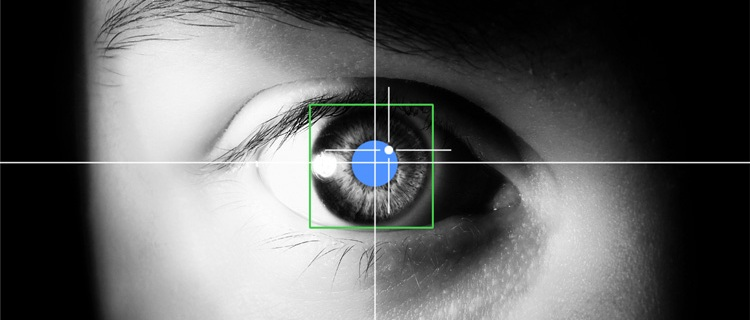
\includegraphics[width=0.60\textwidth]{images/eyetracker.jpg}
\end{figure}
\vspace{0.5 in}
{\centering \huge \color{accentcolor} \sc \textbf{\teamname \\ \productname} \par}
\vspace{0.5 in}
{\centering \large \sc \textbf{\authors} \par}
\newpage


%\vspace{1 in}
%\centerline{January 13th, 2012}
%\newpage

%%% Revision History
\begin{versionhistory}
  	\vhEntry{0.1}{11.18.2015}{KM | JS | ZA | FN | JT}{Created Document}
  	%\vhEntry{0.2}{10.05.2015}{AT|GH}{complete draft}
  	%\vhEntry{0.3}{10.12.2015}{AT|GH}{release candidate 1}
  	%\vhEntry{1.0}{10.20.2015}{AT|GH|CB}{official release}
  	%\vhEntry{1.1}{10.31.2015}{AL}{added design review requests}
\end{versionhistory}
\newpage

%%% Table of contents
\setcounter{tocdepth}{2}
\tableofcontents
\newpage

%%% List of figures and tables (optional)
\listoffigures
\listoftables
\newpage

\section{Introduction}
%Your introduction should describe your product concept in sufficient detail that the architectural design will be easy to follow. The introduction may include information used in the first sections of your SRS for this purpose. At a minimum, ensure that the product concept, scope and key requirements are described

This product shall have three layers that work in unison to track the pupil of the user. The three layers in our system are the Software layer, Daughter Board, and the Cypress CX3. The three layers will be discussed more in the following sections.
\newpage
\section{System Overview}
This section should describe the overall structure of your software system. Think of it as the strategy for how you will build the system. An architectural "layer" is the top-level logical view, or an abstraction, of your design. Layers should be composed of related elements of similar capabilities, and should be highly independent of other layers, but should have very clearly defined interfaces and interactions with other layers. Each layer should be identified individually and should be unique as to its function and purpose within the system. This section should also contain the high-level block diagram of the layers, as shown in the example below, as well as detailed descriptions of the functions of each layer.

\begin{figure}[h!]
	\centering
 	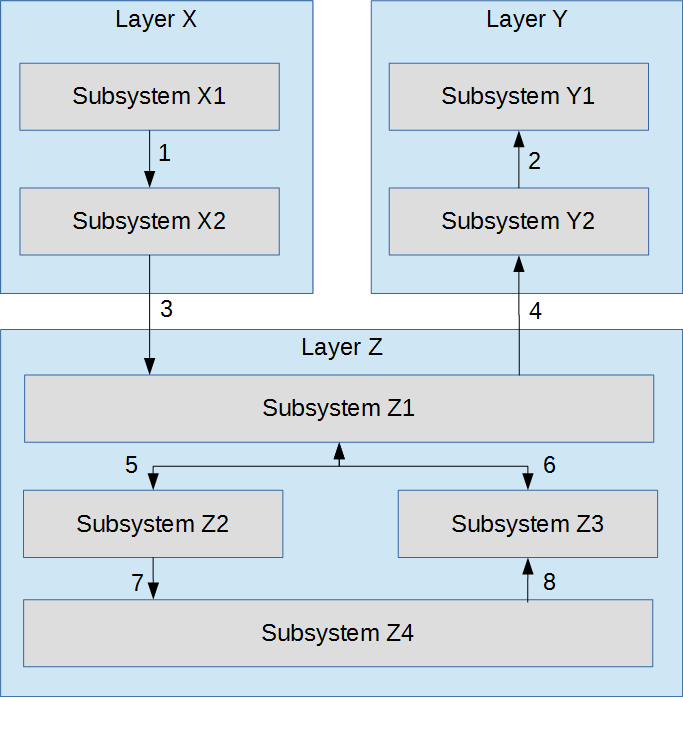
\includegraphics[width=0.60\textwidth]{images/data_flow}
 \caption{A simple architectural layer diagram}
\end{figure}

\subsection{Layer X Description}
Each layer should be described separately in detail. Descriptions should include the features, functions, critical interfaces and interactions of the layer. The description should clearly define the services that the layer provides. Also include any conventions that your team will use in describing the structure: naming conventions for layers, subsystems, modules, and data flows; interface specifications; how layers and subsystems are defined; etc. 

\subsection{Layer Y Description}
Each layer should be described separately in detail. Descriptions should include the features, functions, critical interfaces and interactions of the layer. The description should clearly define the services that the layer provides. Also include any conventions that your team will use in describing the structure: naming conventions for layers, subsystems, modules, and data flows; interface specifications; how layers and subsystems are defined; etc. 

\subsection{Layer Z Description}
Each layer should be described separately in detail. Descriptions should include the features, functions, critical interfaces and interactions of the layer. The description should clearly define the services that the layer provides. Also include any conventions that your team will use in describing the structure: naming conventions for layers, subsystems, modules, and data flows; interface specifications; how layers and subsystems are defined; etc. 
\newpage
\section{Subsystem Definitions \& Data Flow}
%This section breaks down your layer abstraction to another level of detail. Here you grapically represent the logical subsytems that compose each layer and show the interactions/interfaces between those subsystems. A subsystem can be thought of as a programming unit that implements one of the major functions of the layer. It, therefore, has data elements that serve as source/sinks for other subsystems. The logical data elements that flow between subsystems need to be explicitly defined at this point, beginning with a data flow-like diagram based on the block diagram.
The following section shows a high level diagram of all layers of our system.
\begin{figure}[h!]
	\centering
 	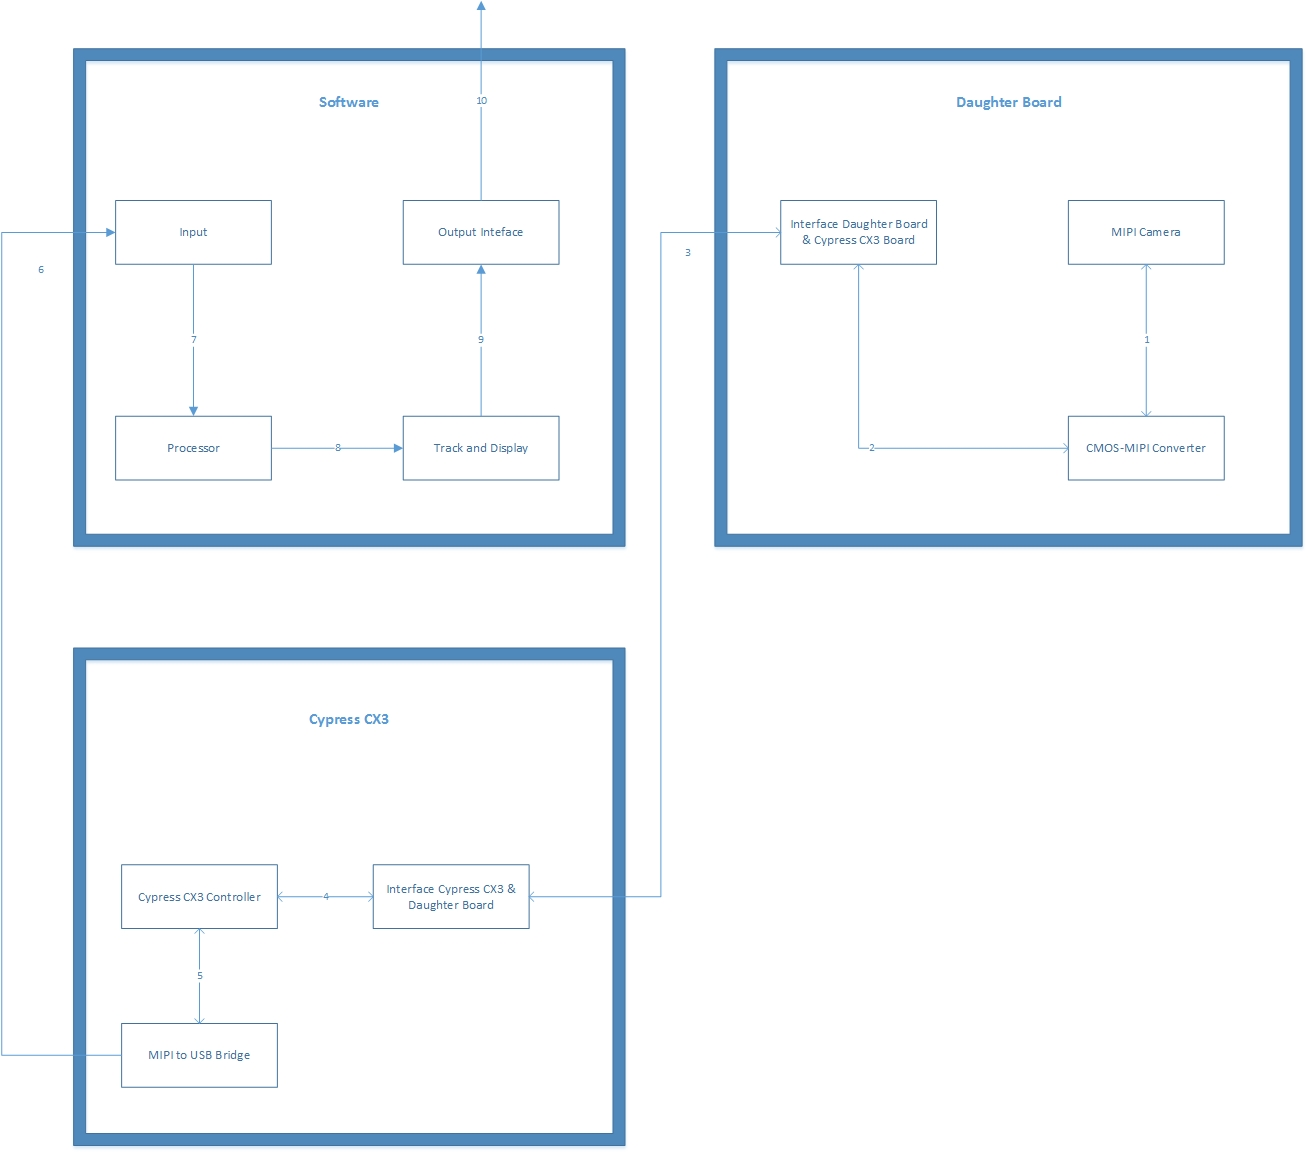
\includegraphics[width=\textwidth]{images/Diagram_WHOLE.jpg}
 \caption{A simple data flow diagram}
\end{figure}

\newpage
\section{X Layer Subsystems}
In this section, the layer is described in some detail in terms of its specific subsystems. Describe each of the layers and its subsystems in a separate chapter/major subsection of this document. The content of each subsystem description should be similar. Include in this section any special considerations and/or trade-offs considered for the approach you have chosen.

\subsection{Subsystem 1}
This section should be a general description of a particular subsystem for the given layer. For most subsystems, an extract of the architectural block diagram with data flows is useful. This should consist of the subsystem being described and those subsystems with which it communicates.

\begin{figure}[h!]
	\centering
 	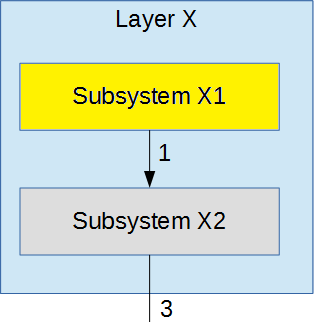
\includegraphics[width=0.60\textwidth]{images/subsystem}
 \caption{Example subsystem description diagram}
\end{figure}

\subsubsection{Assumptions}
Any assumptions made in the definition of the subsystem should be listed and described. Pay particular attention to assumptions concerning interfaces and interactions with other layers.

\subsubsection{Responsibilities}
Each of the responsibilities/features/functions/services of the subsystem as identified in the architectural summary must be expanded to more detailed responsibilities. These responsibilities form the basis for the identification of the finer-grained responsibilities of the layer's internal subsystems. Clearly describe what each subsystem does.

\subsubsection{Subsystem Interfaces}
Each of the inputs and outputs for the subsystem are defined here. Create a table with an entry for each labelled interface that connects to this subsystem. For each entry, describe any incoming and outgoing data elements will pass through this interface.

\begin {table}[H]
\caption {Subsystem interfaces} 
\begin{center}
    \begin{tabular}{ | p{1cm} | p{6cm} | p{3cm} | p{3cm} |}
    \hline
    ID & Description & Inputs & Outputs \\ \hline
    \#xx & Description of the interface/bus & \pbox{3cm}{input 1 \\ input 2} & \pbox{3cm}{output 1}  \\ \hline
    \#xx & Description of the interface/bus & \pbox{3cm}{N/A} & \pbox{3cm}{output 1}  \\ \hline
    \end{tabular}
\end{center}
\end{table}

\subsection{Subsystem 2}
Repeat for each subsystem

\subsection{Subsystem 3}
Repeat for each subsystem


\newpage
\section{Y Layer Subsystems}
\subsection{Interface Daughter Board & Cypress CX3 Board}
The BRD is the interface between the Daughter board and Motherboard.

\begin{figure}[h!]
	\centering
 	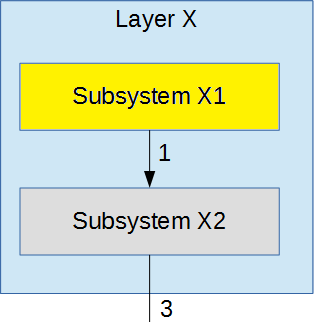
\includegraphics[width=0.60\textwidth]{images/subsystem}
 \caption{Example Daughter Board - BRD diagram}
\end{figure}

\subsubsection{Assumptions}
The BRD should communicate without any issues (like a BUS connection).

\subsubsection{Responsibilities}
The Base BRD Connector is used to interface between the daughter board and the MIPI Camera BRD Connector on the Cypress CX3 Board and vice versa.

\subsubsection{Subsystem Interfaces}
This connector contains 52 pins, but not all of the pins will be used. This connector is directly connected to the camera module connector in order to transfer the data back and forth at a faster rate.  Throughout this connector, multiple pins receive different types of voltages in order to perform different tasks. For complexity issues, the Base BRD Connector will be connected to the bottom layer of the Daughter Board.

\begin {table}[H]
\caption {Subsystem interfaces}
\begin{center}
    \begin{tabular}{ | p{1cm} | p{6cm} | p{3cm} | p{3cm} |}
    \hline
    ID & Description & Inputs & Outputs \\ \hline
     \#01 & MIPI Controls & \pbox{3cm}{Input 1 - SCL \\ Input 2 - SDA} & \pbox{3cm}{Output 1 - MIPI Data \\ Output 2 - MIPI Clock \\ Output 3 - MIPI Power \\ Output 4 - SDA}  \\ \hline
    \end{tabular}
\end{center}
\end{table}

\subsection{MIPI Camera}
The camera module used for the Eye Tracker system is a 5MP pcDuino camera that will be used to capture data for processing. The pcDuino camera uses the OV5640 image sensor.

\begin{figure}[h!]
	\centering
 	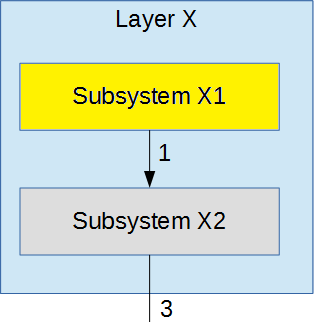
\includegraphics[width=0.60\textwidth]{images/subsystem}
 \caption{Example Daughter Board - Camera Module diagram}
\end{figure}

\subsubsection{Assumptions}
The camera module will capture image and video at least 30FPS at 5MP.

\subsubsection{Responsibilities}
This image sensor is capable of capturing 2592x1944 active array of image and video at a minimum of 30 FPS. Since this new camera uses the OV5640, it is compatible with the Cypress CX3.

\subsubsection{Subsystem Interfaces}

The camera uses the OV5640 image sensor, which is a high quality CMOS image sensor.

\begin {table}[H]
\caption {Subsystem interfaces}
\begin{center}
    \begin{tabular}{ | p{1cm} | p{6cm} | p{3cm} | p{3cm} |}
    \hline
    ID & Description & Inputs & Outputs \\ \hline
    \#01 & CMOS Data from Camera & \pbox{3cm}{Input 1 - SCL \\ Input 2 - SDA} & \pbox{3cm}{Output 1 - Data \\ Output 2 - Clock \\ Output 3 - SDA}  \\ \hline
    \end{tabular}
\end{center}
\end{table}

\subsection{CMOS-MIPI Converter}
The camera connector is new, and will be replacing the camera connector that was on the CX3 development board. The new connector allows for the use of the pcDuino camera module. This where the camera performs a CMOS to MIPI conversion in order to transfer the data collected from the camera module.

\begin{figure}[h!]
	\centering
 	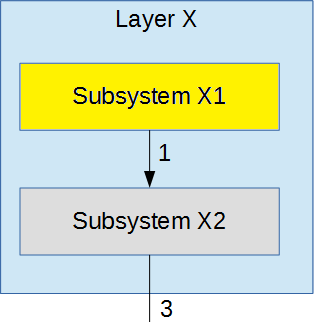
\includegraphics[width=0.60\textwidth]{images/subsystem}
 \caption{Example Daughter Board - Camera Connector diagram}
\end{figure}

\subsubsection{Assumptions}
The camera connector is compatible with the new module and the BRD.

\subsubsection{Responsibilities}
The camera connector is used to connect the camera module to the daughter board and transfer the data that the camera captures to the Base BRD Connector.

\subsubsection{Subsystem Interfaces}
In order for the camera module to function properly with the Cypress CX3, it received different voltage inputs in different pins. The datasheet of the OV5640 (Image Sensor) in order to determine which pins will be used on the camera connector and where to connect each pin at the Base BRD Connector. Since this camera will only be used for eye tracking purposes only, the user will not be able to reset the camera since we disabled the reset pin on the camera connector.

\begin {table}[H]
\caption {Subsystem interfaces}
\begin{center}
    \begin{tabular}{ | p{1cm} | p{6cm} | p{3cm} | p{3cm} |}
    \hline
    ID & Description & Inputs & Outputs \\ \hline
    \#01 & Camera Connector & \pbox{3cm}{Input 1 - MIPI Data \\ Input 2 - MIPI Clock \\ Input 3 - SDA} & \pbox{3cm}{Output 1 - Converted Data \\ Output 2 - Camera Clock Signal \\ Output 3 - SDA}  \\ \hline
    \end{tabular}
\end{center}
\end{table}

\newpage
\section{Z Layer Subsystems}
In this section, the layer is described in some detail in terms of its specific subsystems. Describe each of the layers and its subsystems in a separate chapter/major subsection of this document. The content of each subsystem description should be similar. Include in this section any special considerations and/or trade-offs considered for the approach you have chosen.

\subsection{Subsystem 1}
This section should be a general description of a particular subsystem for the given layer. For most subsystems, an extract of the architectural block diagram with data flows is useful. This should consist of the subsystem being described and those subsystems with which it communicates.

\begin{figure}[h!]
	\centering
 	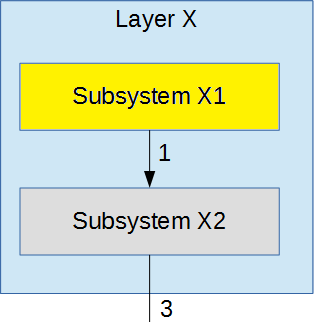
\includegraphics[width=0.60\textwidth]{images/subsystem}
 \caption{Example subsystem description diagram}
\end{figure}

\subsubsection{Assumptions}
Any assumptions made in the definition of the subsystem should be listed and described. Pay particular attention to assumptions concerning interfaces and interactions with other layers.

\subsubsection{Responsibilities}
Each of the responsibilities/features/functions/services of the subsystem as identified in the architectural summary must be expanded to more detailed responsibilities. These responsibilities form the basis for the identification of the finer-grained responsibilities of the layer's internal subsystems. Clearly describe what each subsystem does.

\subsubsection{Subsystem Interfaces}
Each of the inputs and outputs for the subsystem are defined here. Create a table with an entry for each labelled interface that connects to this subsystem. For each entry, describe any incoming and outgoing data elements will pass through this interface.

\begin {table}[H]
\caption {Subsystem interfaces} 
\begin{center}
    \begin{tabular}{ | p{1cm} | p{6cm} | p{3cm} | p{3cm} |}
    \hline
    ID & Description & Inputs & Outputs \\ \hline
    \#xx & Description of the interface/bus & \pbox{3cm}{input 1 \\ input 2} & \pbox{3cm}{output 1}  \\ \hline
    \#xx & Description of the interface/bus & \pbox{3cm}{N/A} & \pbox{3cm}{output 1}  \\ \hline
    \end{tabular}
\end{center}
\end{table}

\subsection{Subsystem 2}
Repeat for each subsystem

\subsection{Subsystem 3}
Repeat for each subsystem


\newpage

%%% References
\bibliographystyle{plain}
\bibliographystyle{reference/IEEEtran_custom}
\bibliography{reference/refs}{}

\end{document}